\documentclass{article}
\usepackage{graphicx} % Required for inserting images
\usepackage{tabularx}
\usepackage{float}
\usepackage{listings}
\usepackage{color}

\definecolor{dkgreen}{rgb}{0,0.6,0}
\definecolor{gray}{rgb}{0.5,0.5,0.5}
\definecolor{mauve}{rgb}{0.58,0,0.82}

\lstset{frame=tb,
  language=VHDL,
  aboveskip=3mm,
  belowskip=3mm,
  showstringspaces=false,
  columns=flexible,
  basicstyle={\small\ttfamily},
  numbers=none,
  numberstyle=\tiny\color{gray},
  keywordstyle=\color{blue},
  commentstyle=\color{dkgreen},
  stringstyle=\color{mauve},
  breaklines=true,
  breakatwhitespace=true,
  tabsize=3
}





\title{Mid-project Report}

% Michael Cooke - 13244785, Raul Lyons - 24565184, Jay Tinsley - 24567707
\author{Jay Tinsley - 24567707 \\ Michael Cooke - 13244785 \\ Raul Lyons - 24565184}


\date{September 2024}

\begin{document}

\maketitle

\section{Description of project}
\subsection{Project Aims}
The purpose of the project is display the output of a sensor to a screen via VGA. This will be achieved by ingesting the direct input into an Arduino, then using an I2C bus to communicate with the FPGA. After the input information is on the FPGA some processing will be done, then the output will be transformed to a VGA output and will be displayed to a monitor.\\

During development simulated wave-forms will be generated on the Arduino until input devices can be tested. This functionality will be toggled in the final product via a control signal (button press).\\

\subsection{Project Diagram}
\begin{figure}[H]
    \centering
    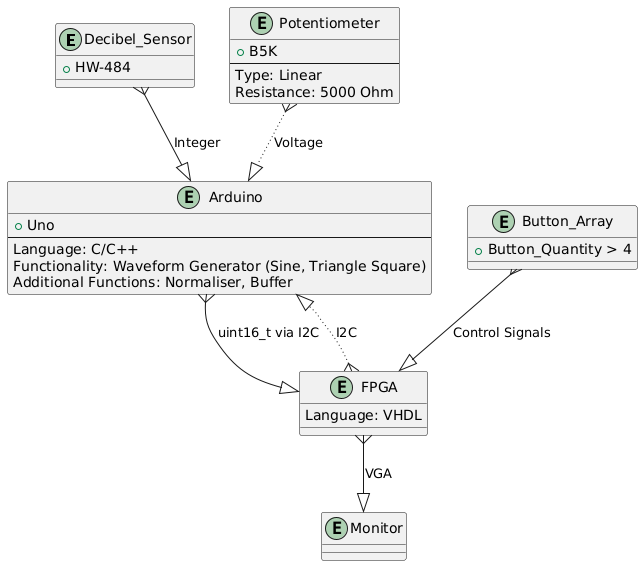
\includegraphics[width=\textwidth, height=0.5\paperheight]{UML_Flowchart.png}
\end{figure}
% @startuml

% entity Decibel_Sensor {
%   +HW-484
% }

% entity Potentiometer {
%   +B5K
%   --
%   Type: Linear
%   Resistance: 5000 Ohm
% }

% entity Arduino {
%   +Uno
%   --
%   Language: C/C++
%   Functionality: Waveform Generator (Sine, Triangle Square)
%   Additional Functions: Normaliser, Buffer 
% }

% entity FPGA {
%   Language: VHDL
% }

% entity Button_Array {
%   +Button_Quantity > 4
% }

% entity Monitor {}

% Decibel_Sensor }--|> Arduino : "Integer”
% Potentiometer }-[dotted]-|> Arduino : "Voltage”
% Arduino }--|> FPGA: "uint16_t via I2C"
% FPGA }-[dotted]-|> Arduino: "I2C"
% Button_Array }--|> FPGA: "Control Signals"
% FPGA }--|> Monitor: "VGA"

% @enduml
\newpage
\subsection{Functionality}
\subsubsection{Arduino}
The Arduino servers two key purposes, the creation and/or ingestion of data and the transmission to the FPGA.\\

Due to the structure of I2C two types of variables were available, either 16 or 8 bit integers. As the intention is to render a 640p x 480p image the 8 bit option was decided against as it would reduce fidelity due to having to upscale the incoming data on the FPGA side. When combined with the HW484 sensor's analog output returning very high values when the sensor is configured to be sensitive, it became apparent that we would have to introduce normalisation to transform outputs to the appropriate ranges.\\

To do this min-max feature scaling is used:\\
\begin{displaymath}
    \centering
    X` = min + \frac{X - X_{min}}{X_{max} - X_{min}} * (max - min)
\end{displaymath}

Additionally, it quickly became apparent that running the I2C communication and data collection synchronously would not be ideal due to the difficulty of maintaining even collection intervals and working from the negotiated clock when extending to bi-directional communication. Therefore, data collection was moved to an interrupt service routine (ISR) and circular buffer was implemented to enabled as much flexibility as possible moving forward.\\
\newpage
\subsubsection{FPGA}
The FPGA board will be used to handle the transformation of the integer input into a Binary map that also implements the circular buffer method of data storage, This map is a real time storage of the display screen, where 1 represents the pixel being on and vice versa. This map will be used by the pixel generator, using the x and y coordinates of the next pixel from the VGA driver, the pixel generator will access the Binary map at that index and pass the value to the VGA driver. \\\\
The VGA driver’s function is synchronizing the horizontal and vertical signals, These synchronization signals, known as Hsync (horizontal sync) and Vsync (vertical sync), these coordinate the update of pixels on the screen.\\\\
The VGA hardware transmits RGB pixel values to the monitor, which are displayed as horizontal scan lines. These lines are drawn from left to right, one by one, and once a line is completed, the scan progresses to the next line vertically, until the entire frame is rendered.\\\\
The Hsync signal marks the end of each horizontal scan line and initiates the blanking region, instructing the display to prepare for the next line. Similarly, Vsync signals the end of a frame and starts the vertical blanking interval, marking the beginning of a new frame. The driver configures these signals based on the display’s resolution and refresh rate, maintaining proper timing to avoid visual distortions like flickering or screen tearing.\\\\

    \begin{center}
        \includegraphics[width=1\linewidth]{protocol.png}
    \end{center}

\subsubsection{I2C Bus}
Data from the Arduino’s sensor is sent to the FPGA through an I2C (Inter-integrated circuit) bus. This protocol uses only two lines, one for the clock (SCL) and one for the data (SDA). The Arduino uno will act as the master device that will initiate the connection with the FPGA and then send data continuously to the FPGA. A state machine is used in the FPGA to properly follow the instructions of the Arduino. The recorded values from the sensor will be sent as 2 bytes of unsigned integers. The data will be stored in a circular buffer before being processed by the VGA driver.  I2C can be used bidirectionally, but for now we will only be sending data one way.\\\\
I2C protocol on Arduino side:\
\begin{enumerate}
    \item The Arduino initiates communication by sending a start condition (Pulling down the SDA line while the SCL is high).
    \item The Arduino then sends a 7-bit address identifying the FPGA as the device that will be communicated with.
    \item Another bit is sent to specify that the Arduino will be writing (sending information) to the target device.
    \item The Arduino waits for an acknowledgement bit from the FPGA before sending the first 8-bit data frame.
    \item The Arduino will then continuously send 1 byte of data at a time while waiting for an acknowledgement after each bit. This will continue until the Arduino sends a stop condition, terminating the connection.
\end{enumerate}
I2C protocol on FPGA side:\
\begin{enumerate}
    \item State 0 – Idle and waiting for start condition from Arduino. Once the start condition is received, it transitions to State 1.
    \item Checks to see if the address sent from the Arduino matches the FPGA’s. If it does, it transitions to State 2. Otherwise, it returns to State 0.
    \item State 2 – Waits to see whether the Arduino wants the FPGA to operate in reading or writing mode. As the FPGA is only expected to receive data for now, the state machine returns to State 0 if writing mode is selected.
    \item  If reading mode is selected, the FPGA will then start a loop of receiving 8 bits of data and sending an acknowledgement bit in response until the stop condition is met. To show that is data is being successfully transmitted, the data will be used to control what is displayed on the FPGA’s seven segment display. 
\end{enumerate}

\newpage
\section{Project Progress}
\subsubsection{Arduino}
\begin{enumerate}
    \item Primary input device implemented and tested
    \begin{figure}[H]
    \centering
    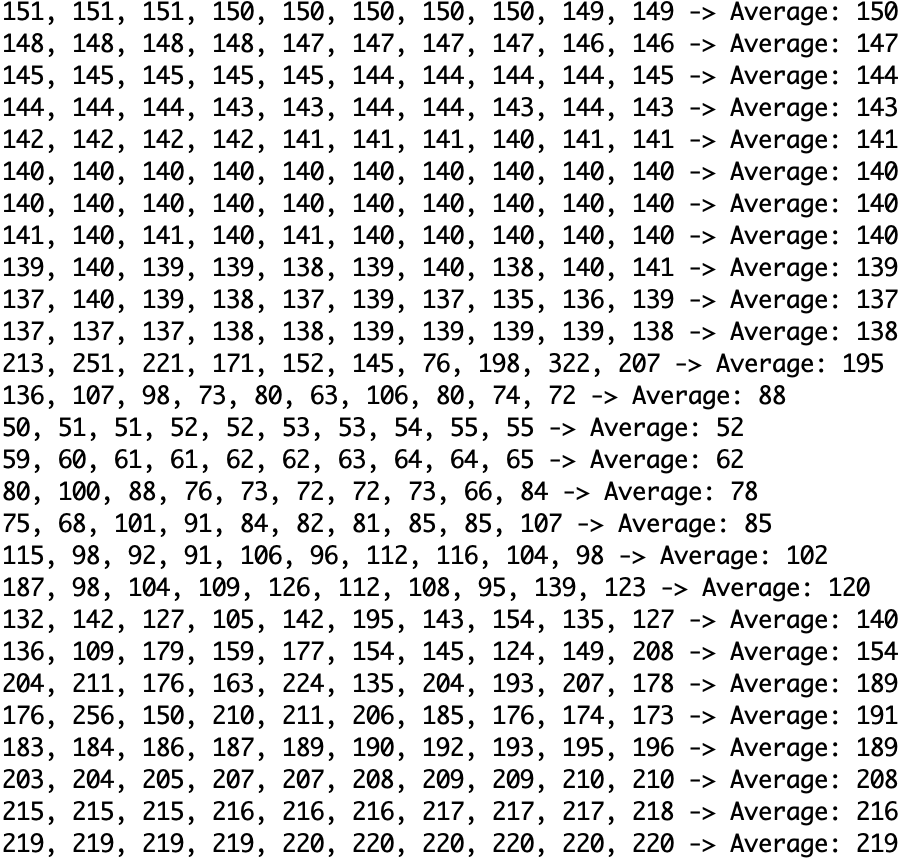
\includegraphics[width=\textwidth, height=0.3\paperheight]{Sensor_Readings.png}
    \end{figure}
    \item ISR implemented $\rightarrow$ Final frequency TBA
    \begin{figure}[H]
    \centering
    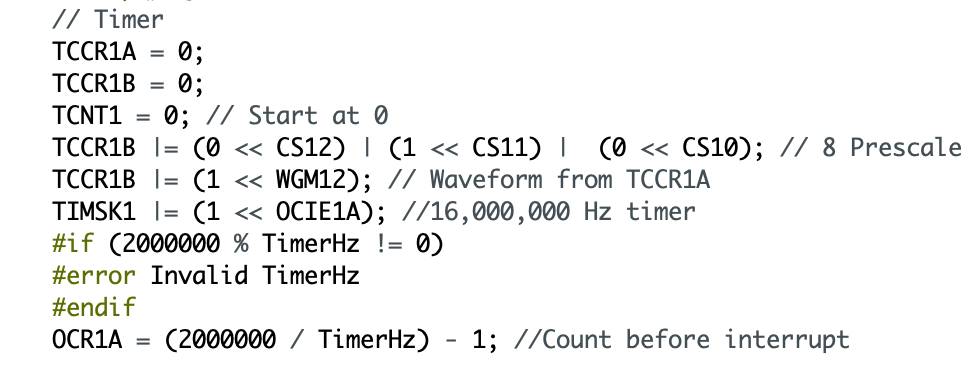
\includegraphics[width=\textwidth, height=0.1\paperheight]{ISR_Code.png}
    \end{figure}
    \item Circular buffer implemented and tested
    \item Normalisation implemented $\rightarrow$ Tuning pending FPGA processing
    \item Waveform Generation (Sine, Square, Triangle) implemented
    \begin{figure}[H]
    \centering
    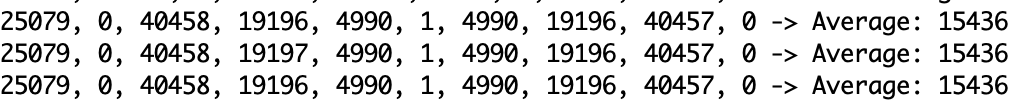
\includegraphics[width=0.75\textwidth, height=0.05\paperheight]{SineWave_Normalised.png}
    \end{figure}
    \item Secondary input device extension $\rightarrow$ Pending
\end{enumerate}

\subsubsection{FPGA}
\begin{enumerate}
    
    \item Uploading and running programs on the board\\
            This step was becoming familiar with the Quartus design software again. 
    \item Clock Divider\\
            The standard operating clock for a VGA driver is 25 Mhz not the 50 MHz that is          
            standard for the Altera board we are using. 
            To work around this a clock divider was made and incorporated using the ALTPLL Wizard in Quartus.\\
    \includegraphics{ClockDivider.png}
    \item VGA driver\\
        Using documentation provided and from online sources i was able to compile a VGA driver with the necessary Input and Output controls for the program. \\
        \includegraphics{VGADriver.png}
    \begin{enumerate}
    \item Pin outs\\
        Using the given Development board pin information spreadsheet file Connections were made with output and input ports\\
        \includegraphics{PinOuts.png}
    \newpage
    \item Basic Screen Connection\\
        First demonstration of the VGA driver working was an implementation of just a whole white screen. Passing a Vcc into the pixel\_on input allowed me to test whether there was valid communication from the FPGA board to the screen\\
            \begin{enumerate}
                \item Issue\\
                    An issue i had at this step was forgetting / not noticing that the default value of an input Pin in Quartus Block Designer is a 1 and not a 0, this meant that the input value for my RST Port in my VGA driver was always High meaning that there was never anything on the screen as the driver was being reset every clock cycle, this was fixed by either placing a NOT gate directly after the Input or altering the Default value on the Input Pin Symbol From VCC to GND.
            \end{enumerate}
            \begin{center}
                \includegraphics[width=1\linewidth]{TestBench.png}
                \includegraphics[width=.8\linewidth]{BasicScreenTest.jpg}    
            \end{center}
            
    \newpage        
    \item Coordinate based Screen pattern\\
    In order to familiarise myself with the use of the pixel outputs from the VGA driver i wrote a simple module that would showcase the control of the driver.
        \begin{center}
            \includegraphics[width=1\linewidth]{PixelPatternTets.png}
            \begin{lstlisting}
                module pixel_pattern(
                    input wire [9:0] x,
                    input wire [9:0] y,
                    output reg pixel_on            
                );
                
                always @(*)
                begin
                    // Top-left quadrant (x < 320 and y < 240) or bottom-right quadrant (x >= 320 and y >= 240)
                    if ((x < 320 && y < 240) || (x >= 320 && y >= 240))
                        pixel_on = 1;  // Turn on the pixel
                    else
                        pixel_on = 0;  // Turn off the pixel
                end
                
                endmodule
            \end{lstlisting}
            \includegraphics[width=.8\linewidth]{PatternScreenTest.jpg}
            
        \end{center}
    \item
    
        
    \end{enumerate}
\end{enumerate}

\subsubsection{I2C}
\begin{enumerate}
    \item Learning about how the I2C protocol works and choosing the best way to program it.
    \begin{enumerate}
        \item As Arduino code was more familiar than VHDL, it was decided that the Arduino will act as the master device, and the FPGA as the slave.
    \end{enumerate}
    \item Writing and upload Arduino code and VHDL code.
    \begin{enumerate}
        \item There were issues found when compiling the FPGA program, to test that that Arduino code works some example VHDL code was used.
        \item The USB-Blaster’s drivers weren’t installed properly so new drivers had to be downloaded before Quartas could program the FPGA.
    \end{enumerate}
    \item Connecting the Arduino to FPGA.
    \begin{enumerate}
        \item The Arduino has dedicated pins for SCL and SDA, which were then connected to 2 general I/O pins on the FPGA, as well as a wire connecting the GND of both boards. The Arduino and FPGA were both powered by a PC through their USB ports.
    \end{enumerate}
\end{enumerate}

\begin{center}
    \includegraphics[width=0.7\textwidth,angle=270]{IMG_1110.jpg}
\end{center}


\section{Timeline}
\begin{tabularx}{\textwidth} { 
  || >{\centering\arraybackslash}c 
  | >{\leftragged\arraybackslash}X | >{\centering\arraybackslash}c || }
\hline
\textbf{Week} & \textbf{Original Tasks } & \textbf{Status}\\ [0.5ex]
\hline
\hline
1 & Subject introduction, group establishment & Completed\\
\hline
2 & Creation of project scaffold, establish git and communication channels & Completed\\
\hline
3 & Complete \textbf{Assessment 1} - Learning Contract, acquire all required materials & Completed\\
\hline
4 & Assign tasks to individual members and research theoretical implementations of I2C and VGA protocols & Completed\\
\hline
5 & Implement POC for Arduino Signal Generation, I2C communication and VGA driver & Completed in Week 6\\
\hline
6 & Prep for and completion of \textbf{Assessment 2} - Project Update & Completed During StuVac\\
\hline
7 & Connect input sensor/s to the Arduino, Establish 2-way IC2 communication, Draw shape via VGA & Arduino and VGA Complete\\
\hline
8 & Integration part 1, Test signal to I2C to VGA to monitor & On Track\\
\hline
9 & Toggle signal, FPGA processing, generalised VGA driver & FPGA processing starting in week 8\\
\hline
10 & Integration part 2, Toggled signal to I2C, FPGA processing, VGA to monitor & On Track\\
\hline
11 & Testing / Buffer week / Opportunity for adding extensions & Similar Expectations\\
\hline
12 & \textbf{Assessment 3} - Project Video and Report & On Track\\
\hline
\end{tabularx}
\end{document}
